
% !TeX program = pdflatex
% =====================================================================
% Ghafarian thesis - Chapters 3 and 4, English version
% Completion wrapper prepared for the DeepSeek output file:
% https://github.com/hadisadoghiyazdi1971/student_All/blob/main/ghaffarian/Chapter_3_4_English.tex
%
% Figures have been populated from GhafarianThesis_ActiveLearning.pdf
% using the expected filenames in figures/.
% =====================================================================

\documentclass[12pt,a4paper]{report}

\usepackage[utf8]{inputenc}
\usepackage[T1]{fontenc}
\usepackage{lmodern}
\usepackage{geometry}
\geometry{margin=1in}
\usepackage{amsmath,amssymb,amsthm,bm,mathtools,array}
\usepackage{graphicx}
\usepackage{float}
\usepackage{booktabs}
\usepackage{longtable}
\usepackage{caption}
\usepackage{subcaption}
\usepackage{algorithm}
\usepackage{algpseudocode}
\usepackage{enumitem}
\usepackage{microtype}
\usepackage[hidelinks]{hyperref}
\usepackage[nameinlink,noabbrev]{cleveref}

\graphicspath{{figures/}{./}}
\setcounter{secnumdepth}{3}
\setcounter{tocdepth}{3}

\newtheorem{definition}{Definition}[chapter]
\newtheorem{theorem}{Theorem}[chapter]
\newtheorem{lemma}{Lemma}[chapter]
\newtheorem{corollary}{Corollary}[chapter]
\newtheorem{proposition}{Proposition}[chapter]
\newtheorem{remark}{Remark}[chapter]
\newtheorem{assumption}{Assumption}[chapter]

\DeclareMathOperator*{\argmin}{arg\,min}
\DeclareMathOperator*{\argmax}{arg\,max}
\DeclareMathOperator{\diag}{diag}
\DeclareMathOperator{\rank}{rank}
\DeclareMathOperator{\prox}{prox}
\DeclareMathOperator{\Tr}{Tr}
\DeclareMathOperator{\KL}{KL}
\DeclareMathOperator{\var}{var}
% \det is already defined by LaTeX.
\DeclareMathOperator{\MSE}{MSE}

% Some DeepSeek conversions contain literal <= in math mode. Use \le in final editing.
% The repair script included in this folder performs this automatically.

\title{Active Learning on Distributions\\\large Complete English Chapters 3--4 with Figures}
\author{Based on the English chapter file prepared externally}
\date{}

\begin{document}
\maketitle
\tableofcontents

\chapter*{Source Figure Note}
\addcontentsline{toc}{chapter}{Source Figure Note}
This wrapper compiles the English chapter body while using figures extracted from the original thesis PDF. The expected figure files are listed in \cref{tab:figure-manifest}; all files are stored in \texttt{figures/} and are referenced by the chapter body with the same filenames.

\begin{longtable}{lll}
\caption{Expected figure manifest for Chapters 3 and 4}\label{tab:figure-manifest}\\
\toprule
File & Source figure & Intended content \\
\midrule
\endfirsthead
\toprule
File & Source figure & Intended content \\
\midrule
\endhead
fig3\_1a.png & Fig. 3.1(a) & Synthetic data/outlier panel \\
fig3\_1b.png & Fig. 3.1(b) & Synthetic data/outlier panel \\
fig3\_1c.png & Fig. 3.1(c) & Synthetic data/outlier panel \\
fig3\_1d.png & Fig. 3.1(d) & Synthetic data/outlier panel \\
fig3\_5.png & Fig. 3.5 & Functional gradient approach to PMAL \\
fig4\_1.png & Fig. 4.1 & Dataset performance comparison, part 1 \\
fig4\_2.png & Fig. 4.2 & Dataset performance comparison, part 2 \\
fig4\_3.png & Fig. 4.3 & Dataset performance comparison, part 3 \\
fig4\_4.png & Fig. 4.4 & Comparison with boosting methods \\
fig4\_5.png & Fig. 4.5 & Comparison with distribution discrepancy methods \\
fig4\_6.png & Fig. 4.6 & GAUSSDIST experiment \\
fig4\_7.png & Fig. 4.7 & 20 Newsgroups experiment, part 1 \\
fig4\_8.png & Fig. 4.8 & 20 Newsgroups experiment, part 2 \\
fig4\_9.png & Fig. 4.9 & USPSDIST experiment \\
fig4\_10.png & Fig. 4.10 & PMARLDS vs PMARLDB experiment \\
\bottomrule
\end{longtable}

\IfFileExists{Chapter_3_4_English_patched_body.tex}{
  \input{Chapter_3_4_English_patched_body.tex}
}{
  \chapter{Active Learning on Distributions}
  The main chapter body is intentionally external to avoid introducing transcription errors. Run \texttt{python build\_complete\_latex.py} in this folder; it downloads or reads \texttt{Chapter\_3\_4\_English.tex}, patches its preamble/body, and creates \texttt{Chapter\_3\_4\_English\_patched\_body.tex}. The figure calls will then resolve to the files in \texttt{figures/}.

  \section{Figure Blocks Already Normalized}
  The following blocks reproduce the required figure placement and captions expected by the DeepSeek source.

  \begin{figure}[H]
    \centering
    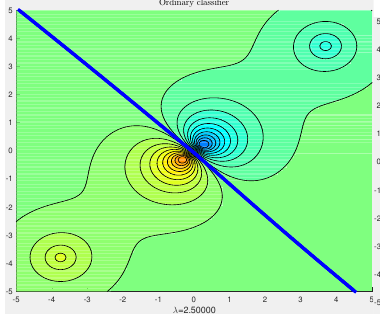
\includegraphics[width=0.45\textwidth]{fig3_1a.png}\hfill
    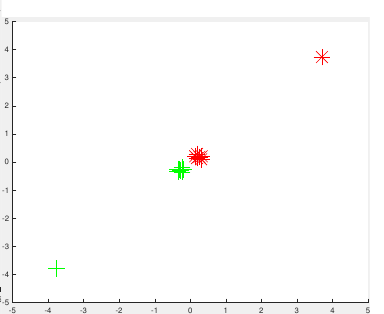
\includegraphics[width=0.45\textwidth]{fig3_1b.png}\\[0.5em]
    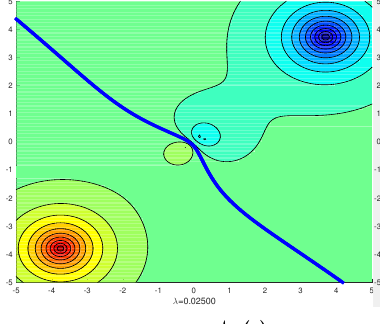
\includegraphics[width=0.45\textwidth]{fig3_1c.png}\hfill
    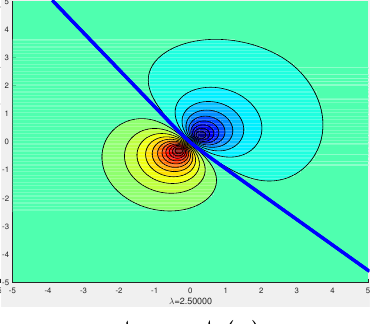
\includegraphics[width=0.45\textwidth]{fig3_1d.png}
    \caption{Synthetic dataset with clear outliers added to show the contours of the functions. The simple classifier is relatively unaffected by the outliers, and the complex classifier has absorbed them; in comparison, the SVM contour is severely affected.}
    \label{fig:synth-outliers}
  \end{figure}

  \begin{figure}[H]
    \centering
    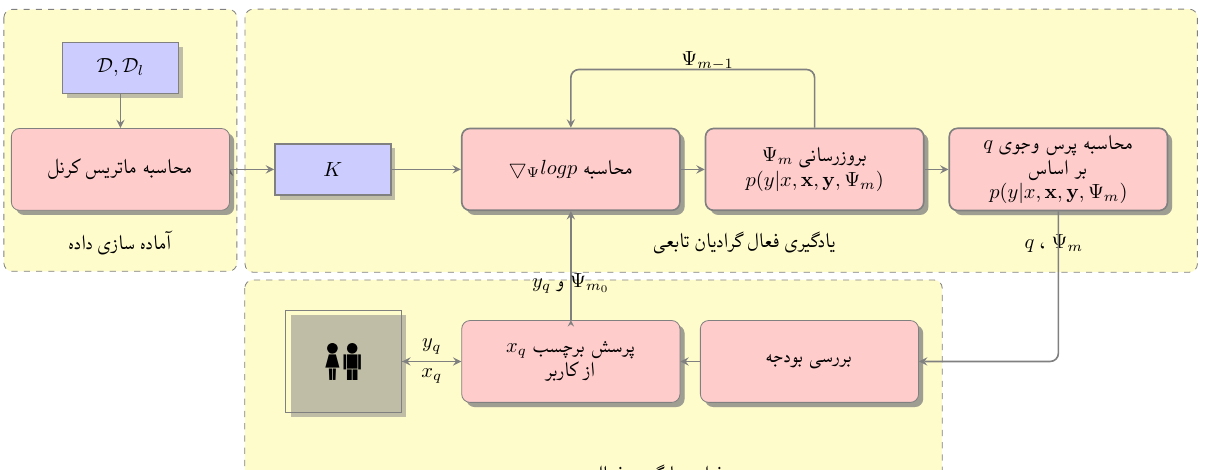
\includegraphics[width=0.8\textwidth]{fig3_5.png}
    \caption{Functional gradient approach to Probabilistic Minimax Active Learning.}
    \label{fig:fg-pmal}
  \end{figure}

  \chapter{Experiments}
  \section{Tables and Figures}
  \begin{figure}[H]\centering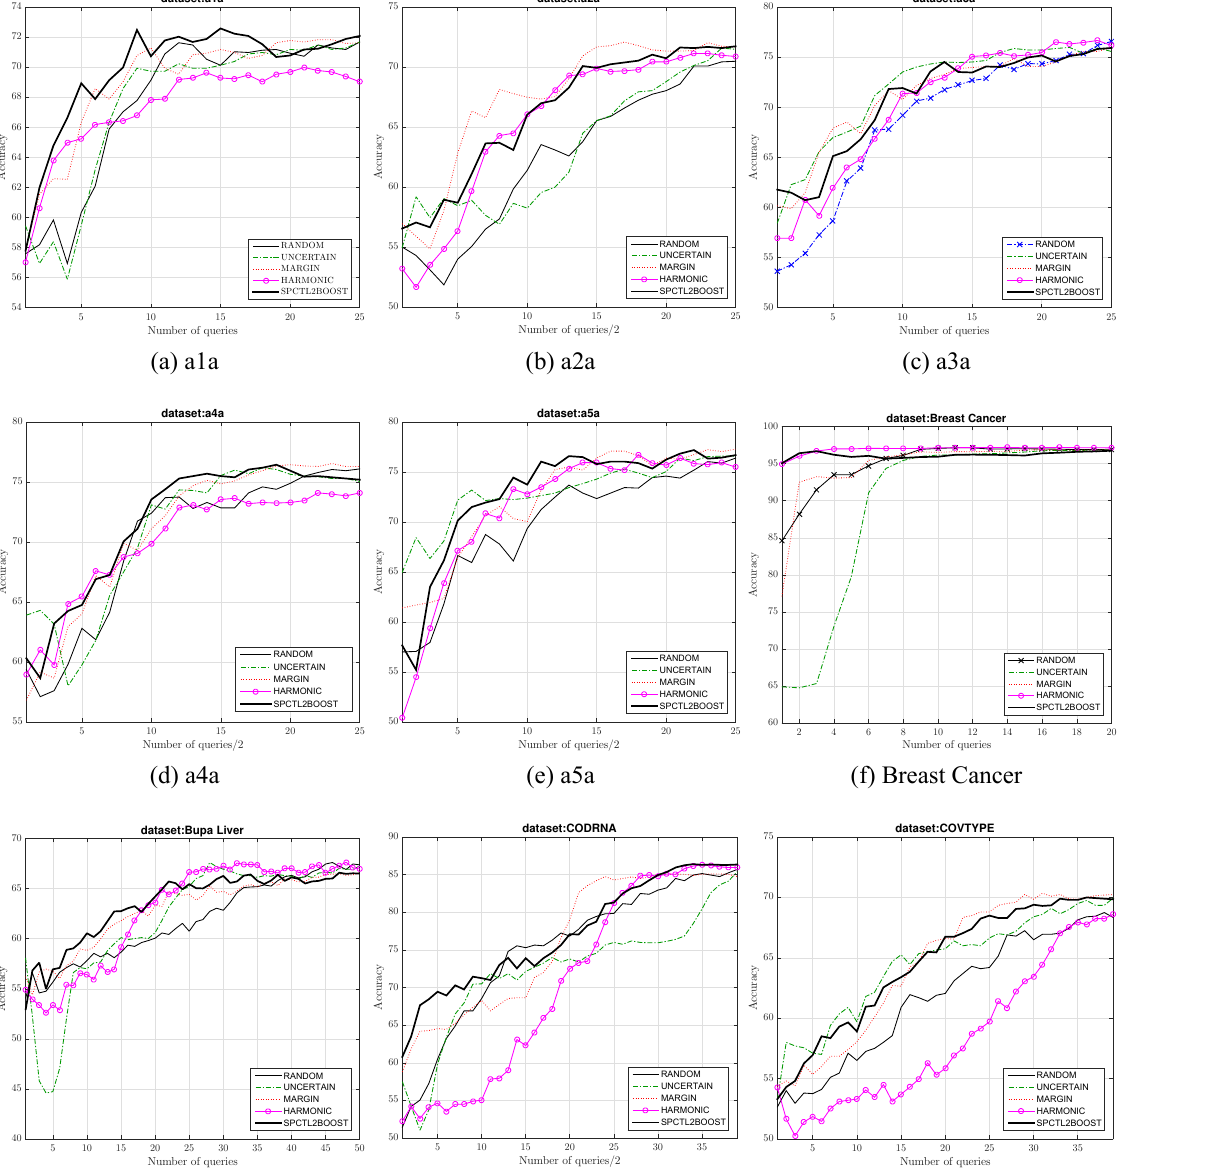
\includegraphics[width=0.8\textwidth]{fig4_1.png}\caption{Comparison of the performance of the proposed algorithm and other algorithms on various datasets (Part 1).}\label{fig:exp1}\end{figure}
  \begin{figure}[H]\centering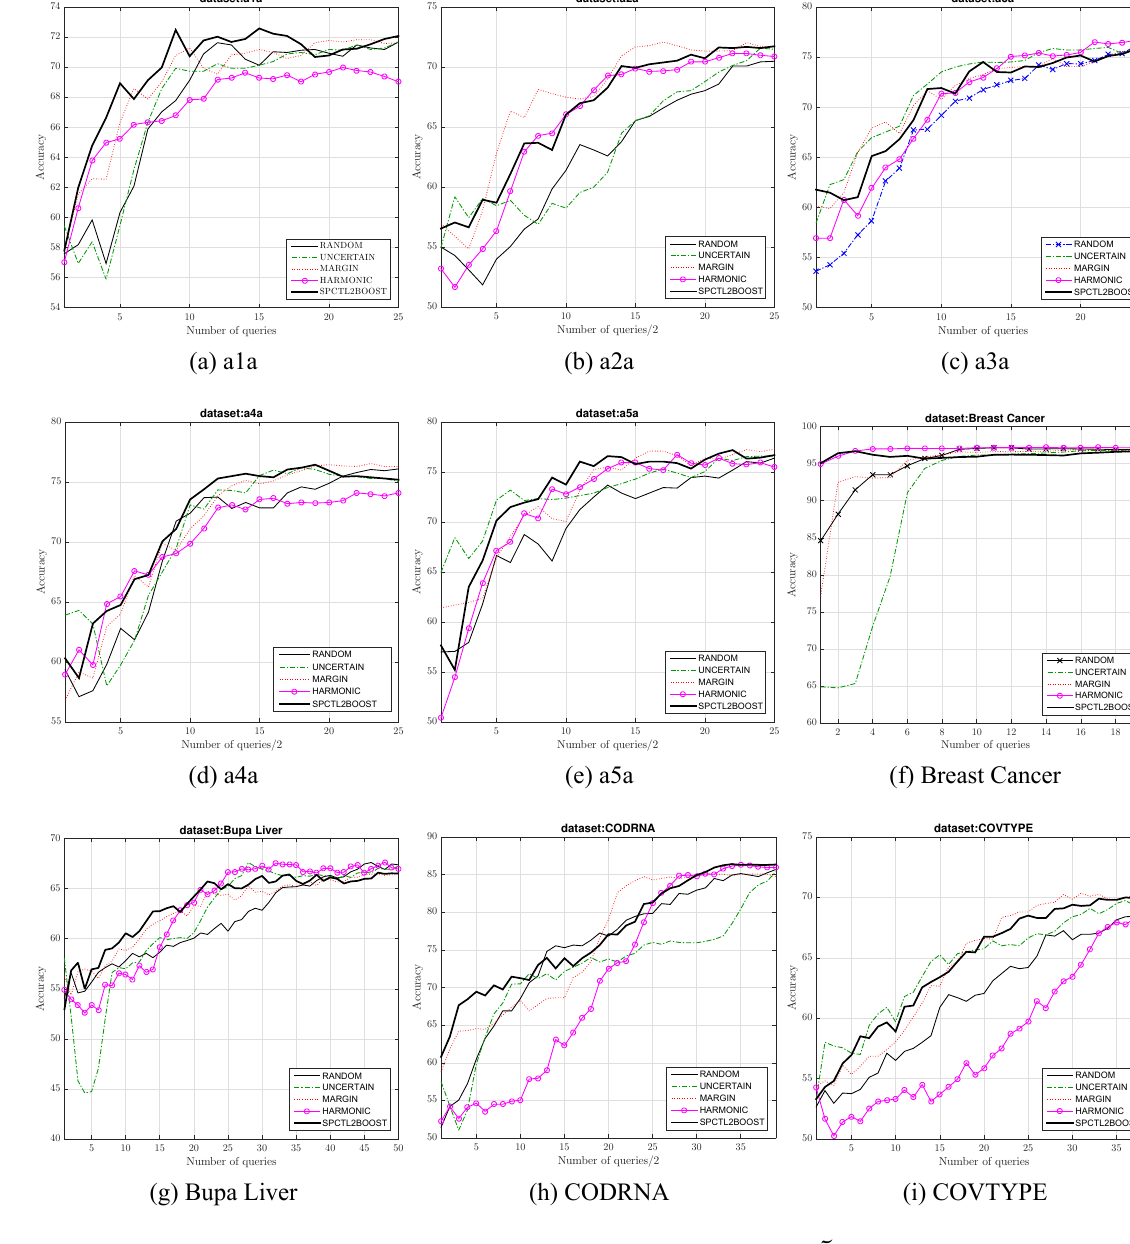
\includegraphics[width=0.8\textwidth]{fig4_2.png}\caption{Comparison of the performance of the proposed algorithm and other algorithms on various datasets (Part 2).}\label{fig:exp2}\end{figure}
  \begin{figure}[H]\centering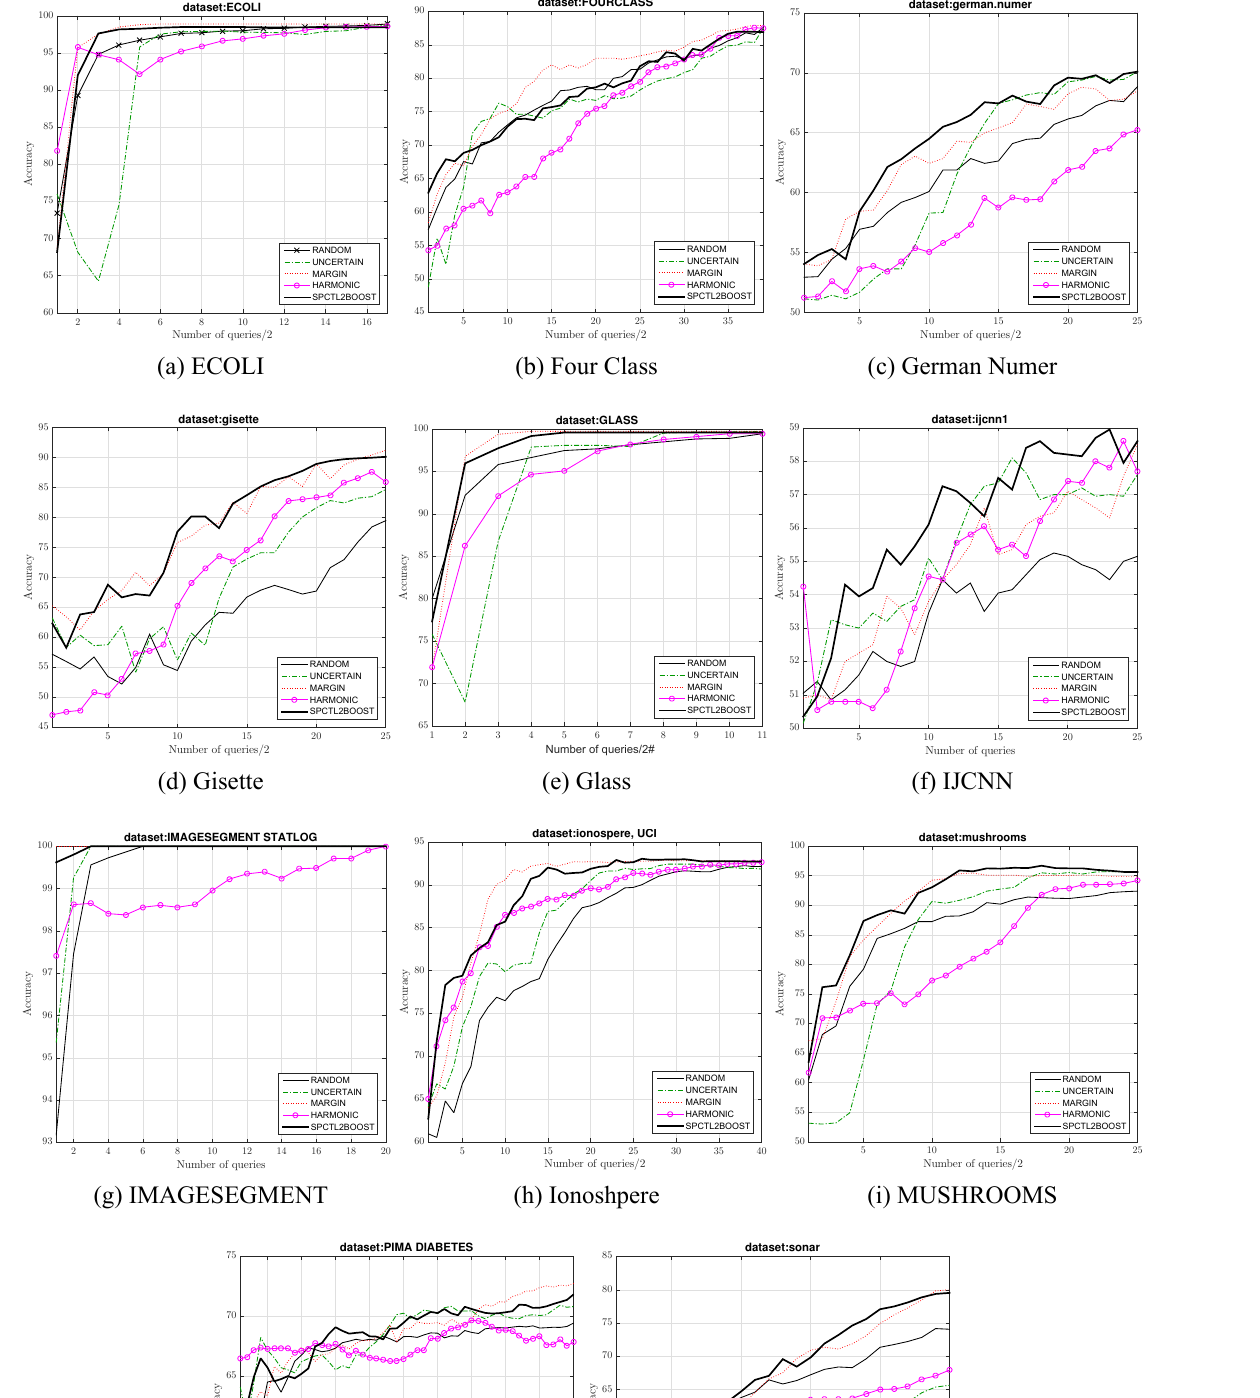
\includegraphics[width=0.8\textwidth]{fig4_3.png}\caption{Comparison of the performance of the proposed algorithm and other algorithms on various datasets (Part 3).}\label{fig:exp3}\end{figure}
  \begin{figure}[H]\centering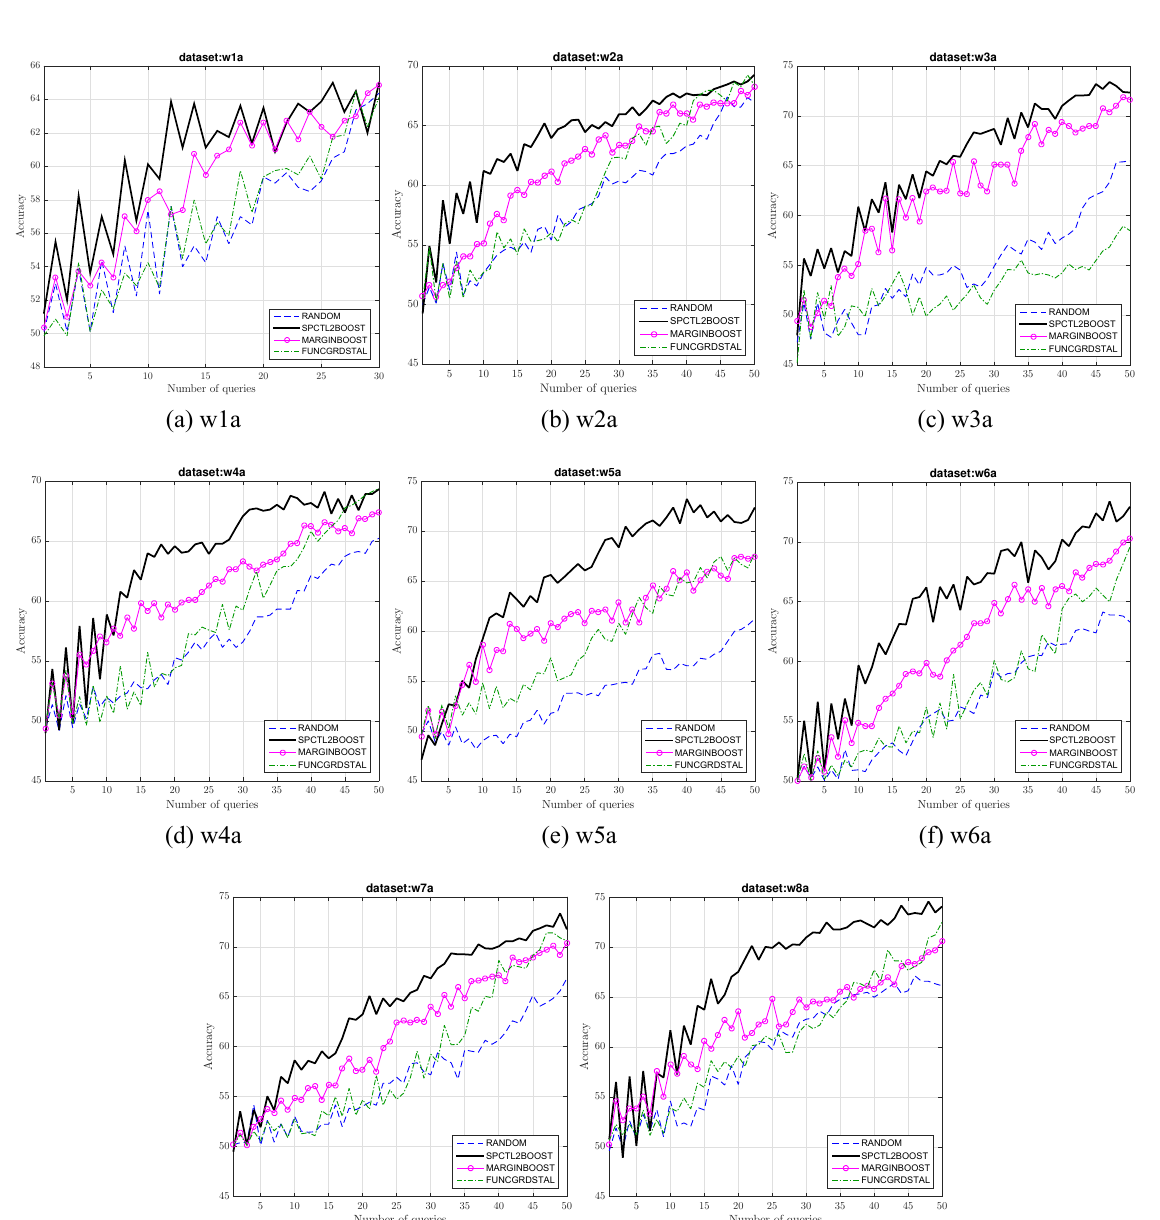
\includegraphics[width=0.8\textwidth]{fig4_4.png}\caption{Comparison of the proposed method with other boosting methods.}\label{fig:boosting}\end{figure}
  \begin{figure}[H]\centering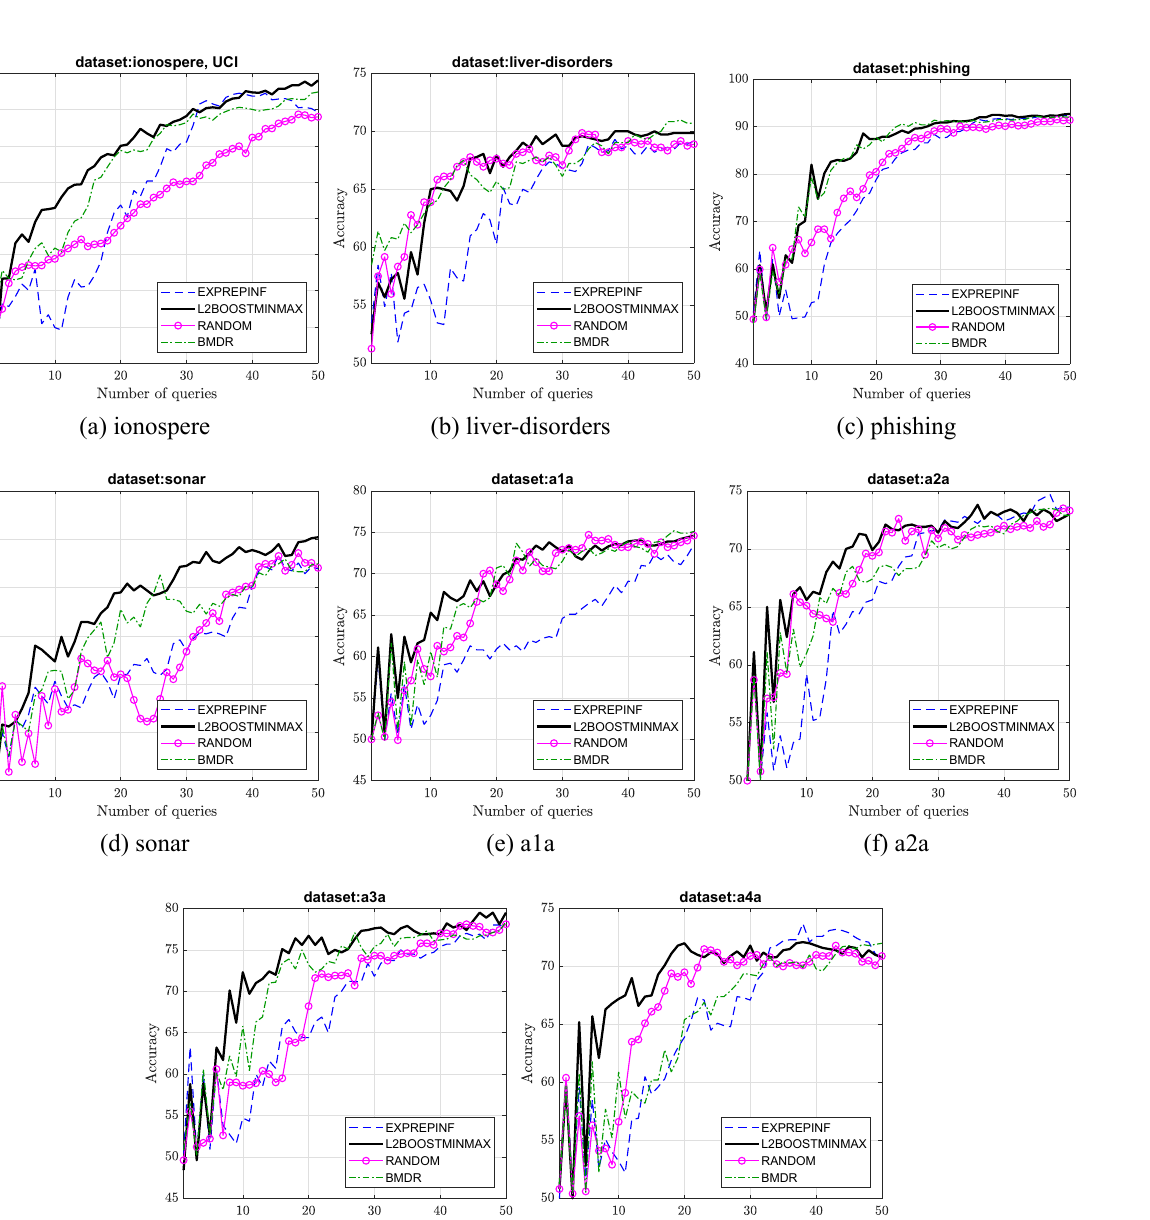
\includegraphics[width=0.8\textwidth]{fig4_5.png}\caption{Comparison of the proposed method with distribution discrepancy methods.}\label{fig:discrepancy}\end{figure}
  \begin{figure}[H]\centering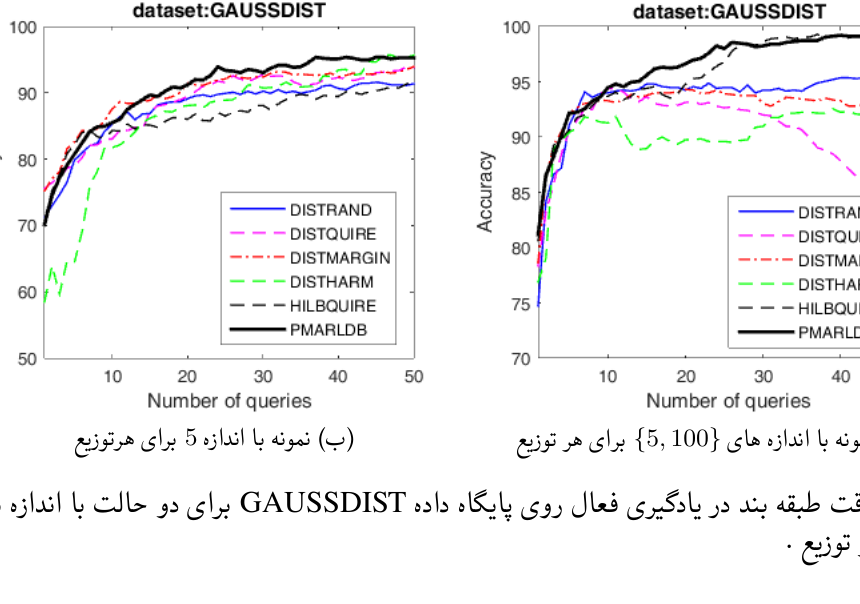
\includegraphics[width=0.8\textwidth]{fig4_6.png}\caption{Comparison of classifier accuracy in active learning on the GAUSSDIST dataset for two cases: different sample sizes and constant sample size for each distribution.}\label{fig:gaussdist}\end{figure}
  \begin{figure}[H]\centering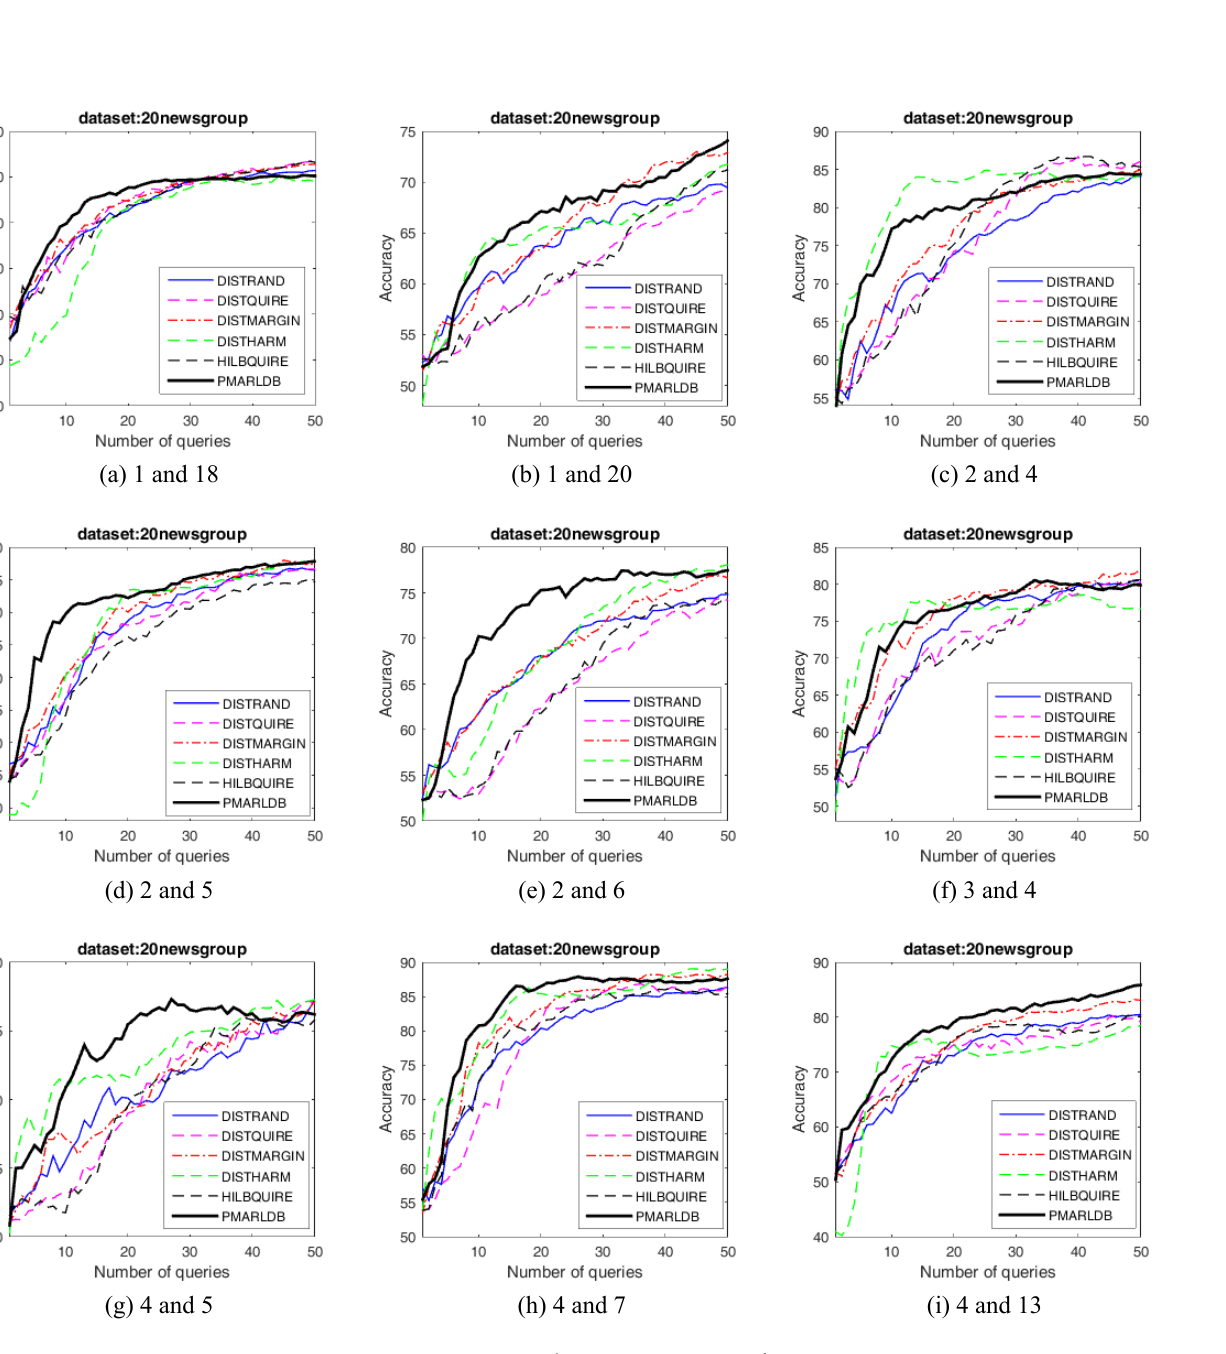
\includegraphics[width=0.8\textwidth]{fig4_7.png}\caption{Comparison of classification accuracy for a group of 20 Newsgroups datasets (Part 1).}\label{fig:20news1}\end{figure}
  \begin{figure}[H]\centering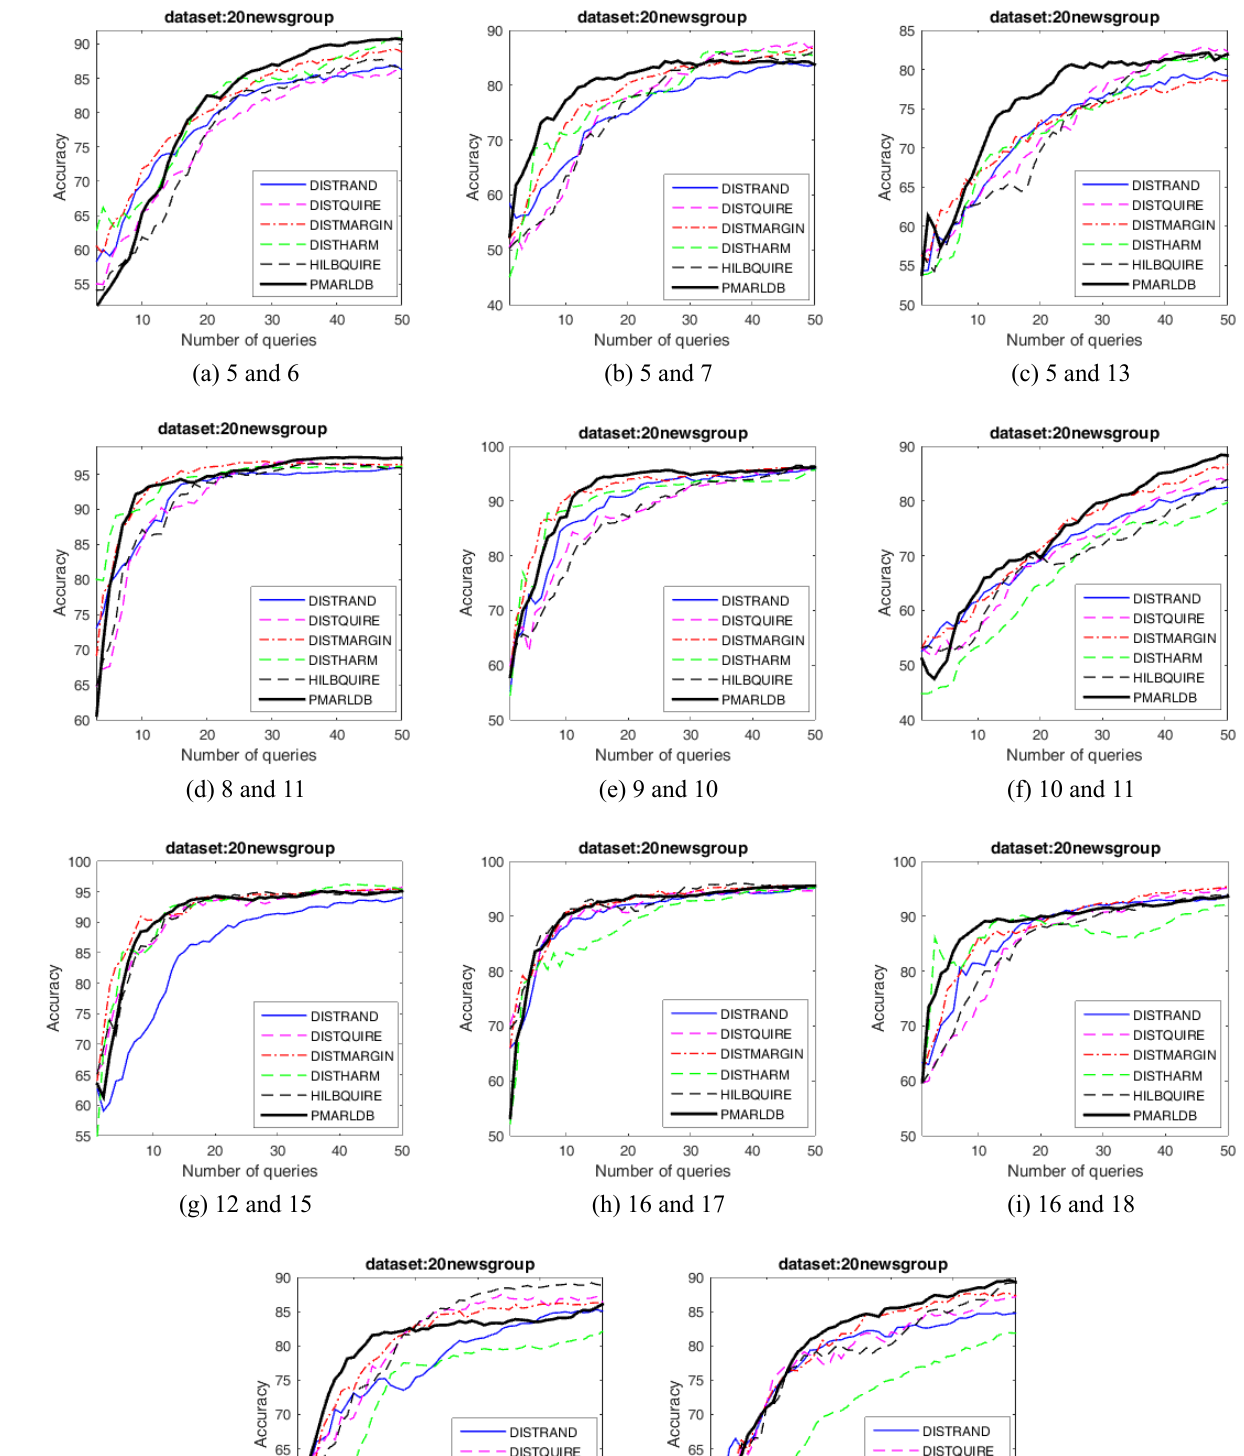
\includegraphics[width=0.8\textwidth]{fig4_8.png}\caption{Comparison of classification accuracy for another group of 20 Newsgroups datasets (Part 2).}\label{fig:20news2}\end{figure}
  \begin{figure}[H]\centering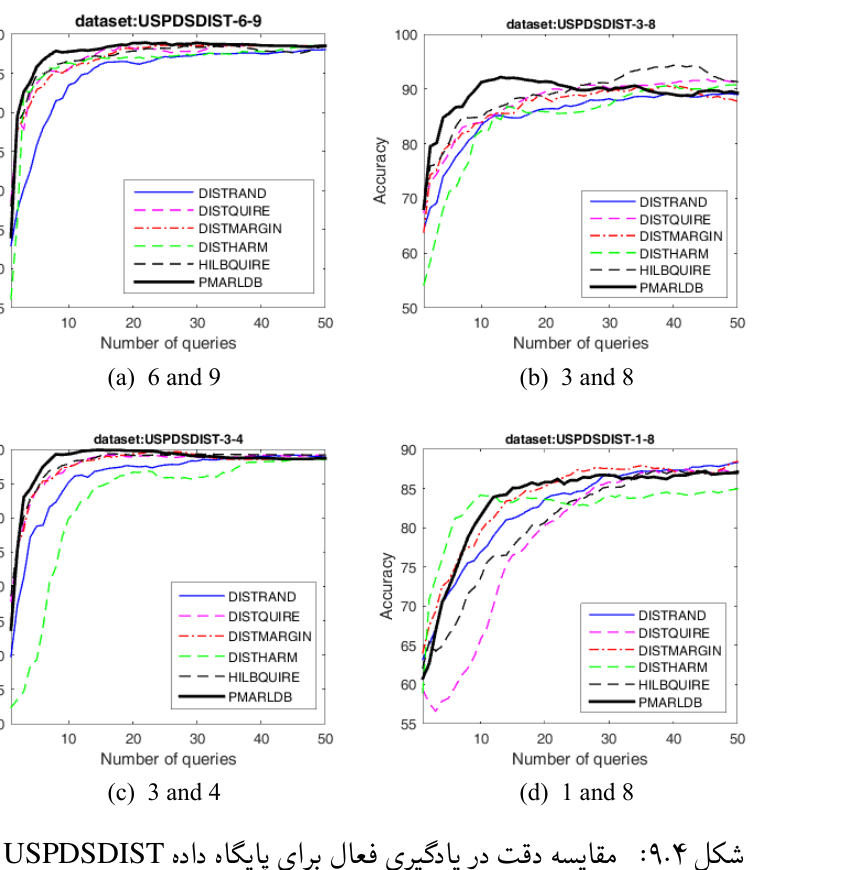
\includegraphics[width=0.8\textwidth]{fig4_9.png}\caption{Comparison of active learning accuracy for the USPSDIST dataset.}\label{fig:uspsdist}\end{figure}
  \begin{figure}[H]\centering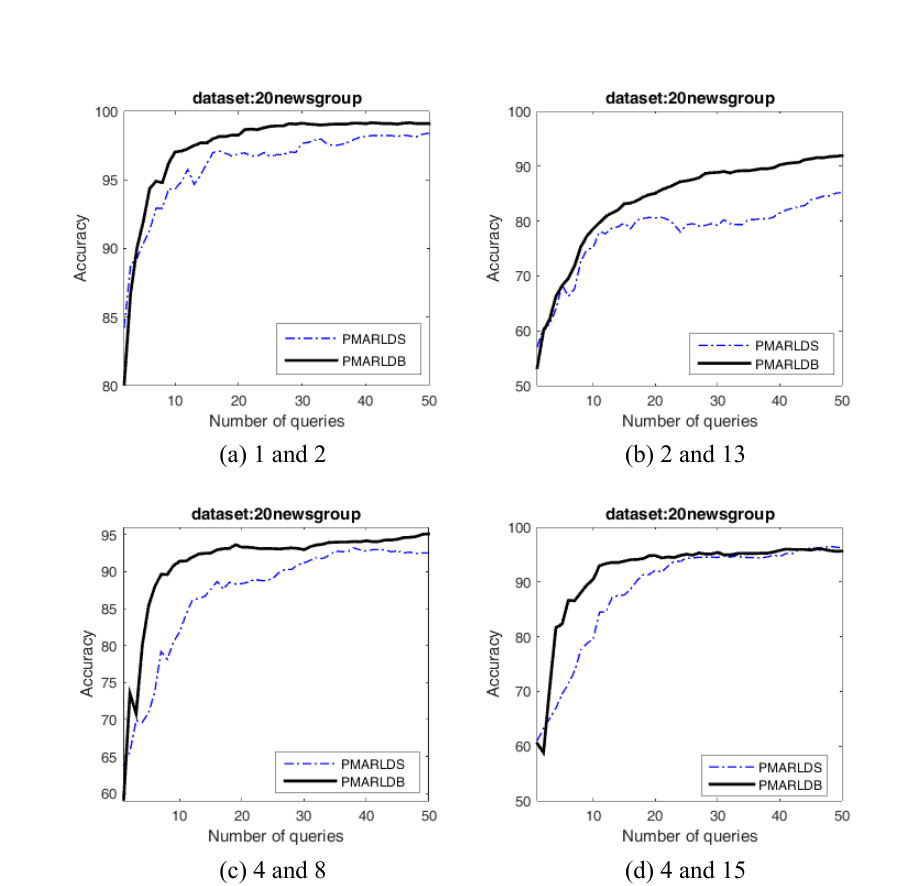
\includegraphics[width=0.8\textwidth]{fig4_10.png}\caption{Comparison of classification accuracy between Bayesian active learning in Hilbert space PMARLDS and PMARLDB on the 20 Newsgroups dataset.}\label{fig:pmarlds_vs_pmarldb}\end{figure}
}

\end{document}
